\title[\LaTeX\ and Web]{Madagascar \\
\LaTeX\ and Web tools}

\author[S. Fomel] % (optional, nur bei vielen Autoren)
{Sergey~Fomel}
% - Der \inst{?} Befehl sollte nur verwendet werden, wenn die Autoren
%   unterschiedlichen Instituten angeh�ren.

\institute[UT Austin] % (optional, aber oft n�tig)
{
  Bureau of Economic Geology \\
  Jackson School of Geosciences \\
  University of Texas at Austin
}

\date[Vancouver School \& Workshop]{August 30, 2006}

\begin{frame}
  \titlepage
\end{frame}

\begin{frame}
  \frametitle{The Big Scheme of Things}
  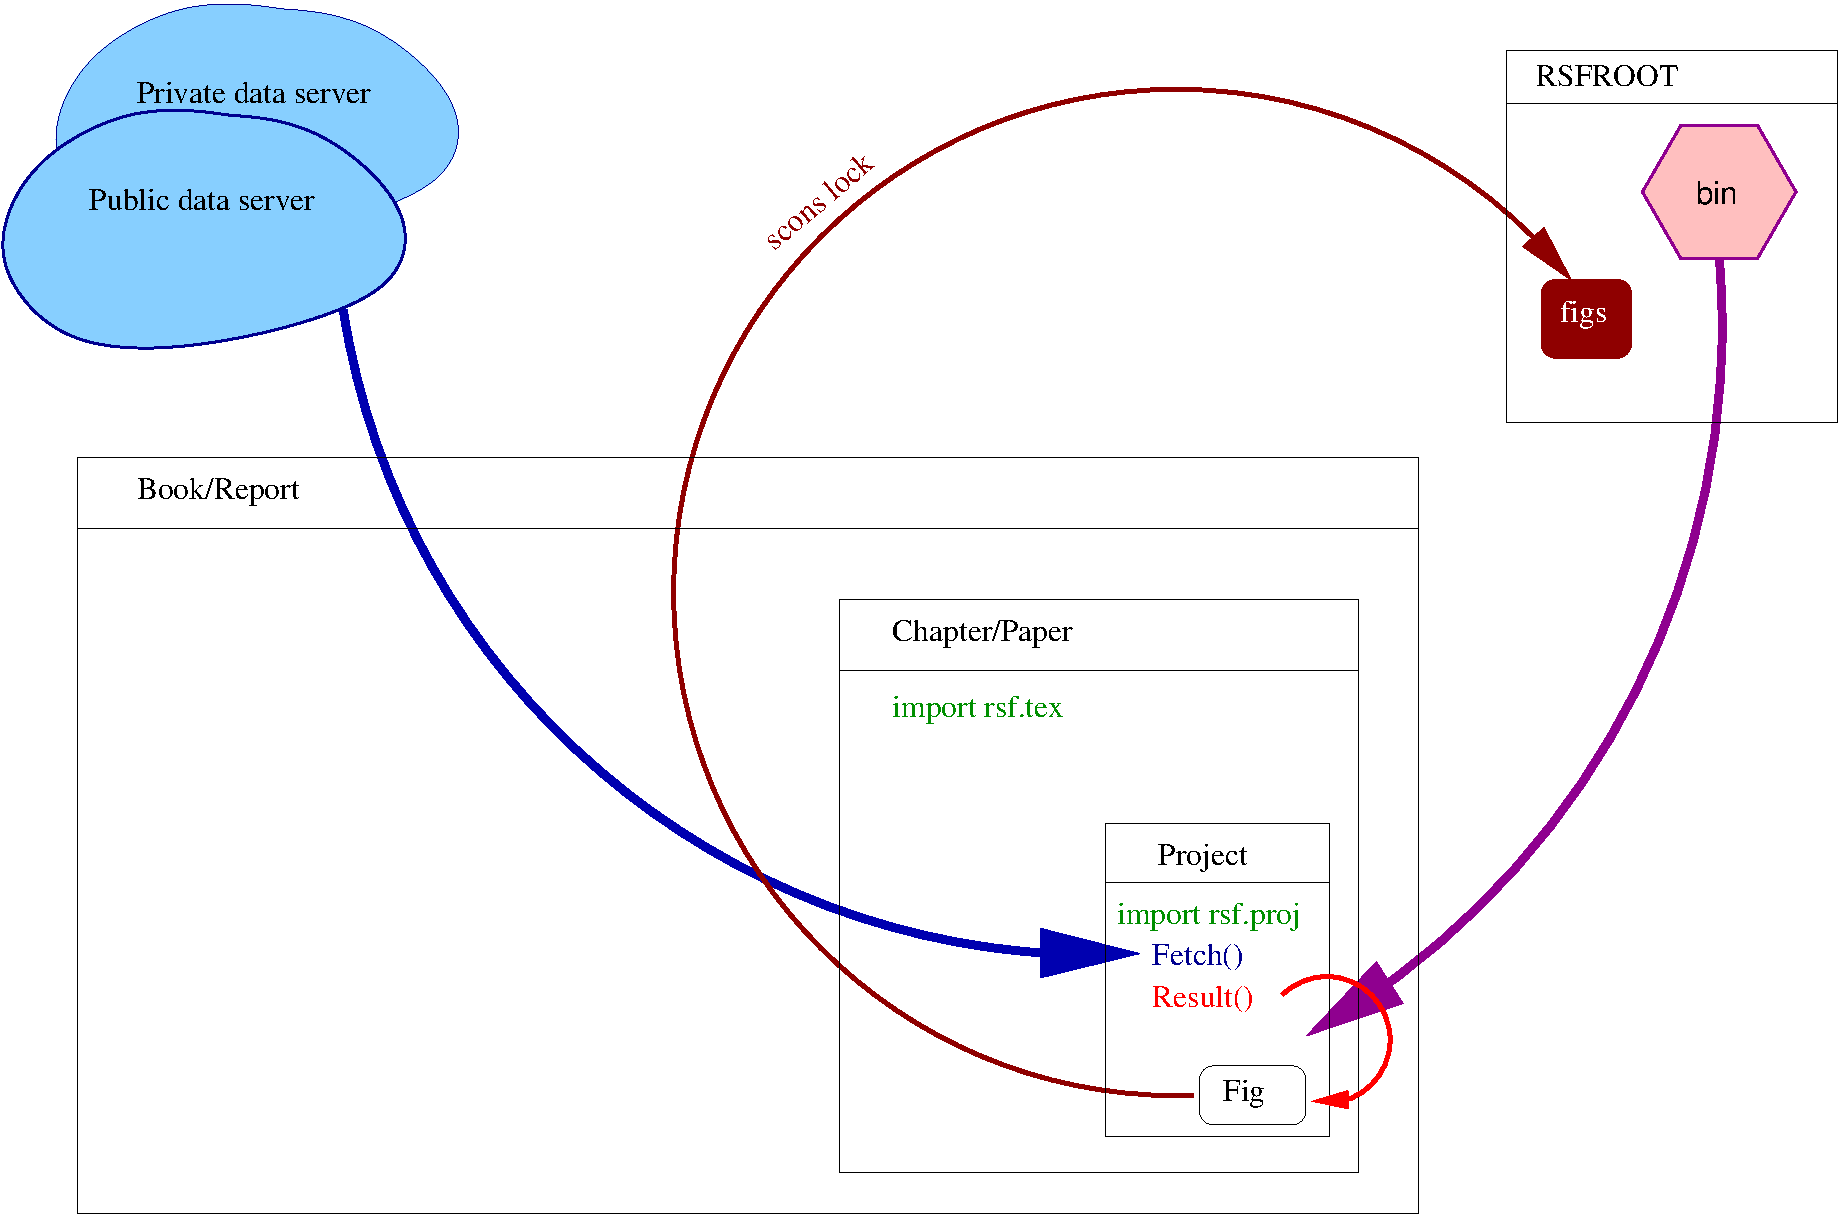
\includegraphics[height=0.8\textheight]{XFig/Fig/scheme}
\end{frame}

\begin{frame}
  \frametitle{The Big Scheme of Things II}
  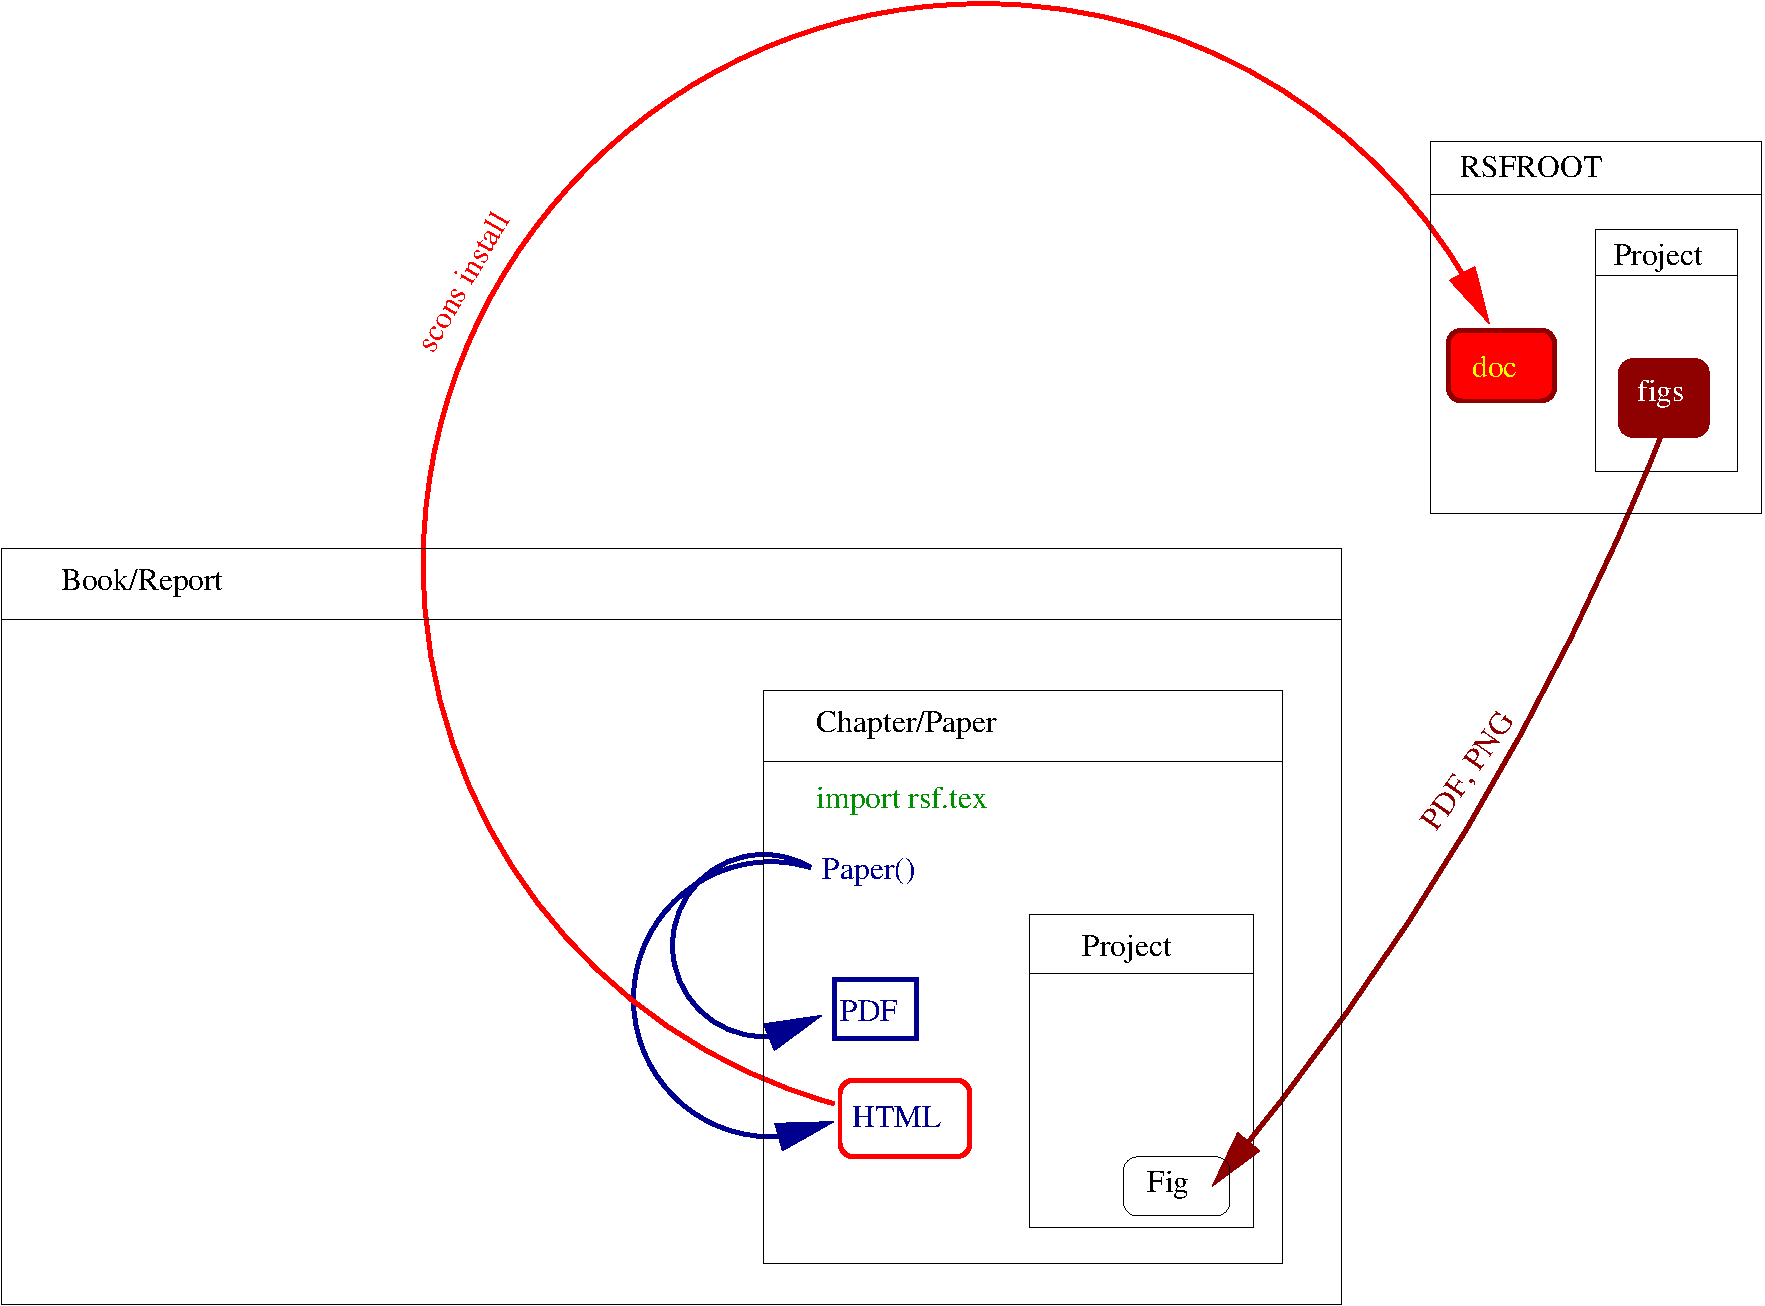
\includegraphics[height=0.8\textheight]{XFig/Fig/scheme2}
\end{frame}

\begin{frame}
  \frametitle{Outline}
  \tableofcontents[pausesections]
\end{frame}

\section{\LaTeX\ tools}
\begin{frame}<beamer>
  \frametitle{Outline}
  \tableofcontents[currentsection]
\end{frame}

\begin{frame}
  \frametitle{{\LaTeX}}
\begin{minipage}{0.45\textwidth}
\centering
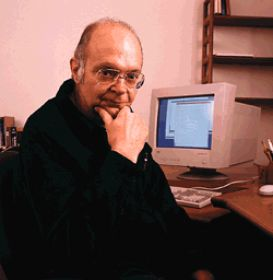
\includegraphics[width=\textwidth]{Fig/knuth.jpg}
\end{minipage}
\hfill
\begin{minipage}{0.45\textwidth}
    \begin{itemize}
    \item Documentation system  
    \item Extends \TeX
    \begin{itemize}
    \item ``Open source''
    \item ``Reproducible''
   \end{itemize}
\item Descriptive language
    \end{itemize}
\end{minipage}
\end{frame}

\begin{frame}
  \frametitle{SEGTeX}
  \begin{itemize}
  \item {\LaTeX2e} package
  \item In development 2001--Present
  \item {\color{blue}{\url{http://segtex.sourceforge.net/}}}
  \item Multiple purpose
    \begin{itemize}
    \item \emph{Geophysics} papers
    \begin{itemize}
    \item Manuscript style
    \item Publication style 
    \end{itemize}
    \item SEG expanded abstracts
    \item Other
    \begin{itemize}
    \item books and reports
    \item EAGE publications
    \item presentations
     \end{itemize}
    \end{itemize}
   \end{itemize}
\end{frame}

\begin{frame}
  \frametitle{Look Inside SEGTeX}
  \begin{itemize}
  \item \texttt{texmf/}
    \begin{itemize}
    \item \texttt{ls-R} (update with \texttt{texconfig rehash}) 
    \item \texttt{tex/latex/seg/}

    \begin{itemize}
    \item \texttt{geophysics.dtx} (literate programming)
    \item \texttt{geophysics.cls}
    \item \texttt{seg.sty}
    \item $\cdots$
    \end{itemize}

    \item \texttt{bibtex/bst/seg/}

     \begin{itemize}
    \item \texttt{seg.bst}
    \item \texttt{seglike.bst} (Joerg Schleicher)
    \end{itemize}

    \item \texttt{bibtex/bib/seg/}

    \begin{itemize}
    \item \texttt{SEG2005.bib}
    \item \texttt{SEG.bib}
    \end{itemize}

    \item {\texttt{latex2html/}}
    
    \begin{itemize}
    \item \texttt{perl/geophysics.perl}
    \item \texttt{icons/}
    \item \texttt{style.css}
    \end{itemize}

    \end{itemize}    
  \end{itemize}
\end{frame}

\begin{frame}
\tiny
\lstset{language=[LaTeX]TeX,showstringspaces=false}
\lstinputlisting[lastline=34,frame=single]{\TEXMF/tex/latex/seg/geophysics_example.ltx}
\normalsize
\end{frame}

\section{From \LaTeX\ to PDF}
\begin{frame}<beamer>
  \frametitle{Outline}
  \tableofcontents[currentsection]
\end{frame}

\begin{frame}
  \frametitle{\LaTeX\ to PDF with SCons}
  \begin{itemize}
  \item \texttt{scons [paper\_name.]ltx}  
\begin{itemize}
\item Add preamble and $\backslash$end\{document\} to \texttt{paper.tex})
  \item Collect figures and convert them to PDF
  \begin{itemize}
  \item Reproducible Vplot from Madagascar
  \item	Conditionally reproducible (MATLAB, Mathematica, XFig, ...)
  \item Non-reproducible 
  \end{itemize}
\end{itemize}
  \item \texttt{scons [paper\_name.]pdf}  
  \begin{itemize}
  \item Generate PDF with \texttt{pdflatex}
  \end{itemize}
  \item \texttt{scons [paper\_name.]read} 
  \begin{itemize}
  \item Display PDF with \texttt{acroread}, \texttt{xpdf}, etc.))
  \end{itemize}	
  \end{itemize}

\tiny
\lstset{language=python,showstringspaces=false}
\lstinputlisting[frame=single]{\TEXMF/tex/latex/seg/SConstruct2}
\normalsize
\end{frame}

\begin{frame}
\tiny
\frametitle{\texttt{SConstruct} examples}
\lstinputlisting[frame=single]{\TEXMF/tex/latex/seg/SConstruct3}
\vfill
\lstinputlisting[firstline=80,lastline=84,frame=single]{SConstruct}
\normalsize
\end{frame}

\section{From \LaTeX\ to HTML}
\begin{frame}<beamer>
  \frametitle{Outline}
  \tableofcontents[currentsection]
\end{frame}

\begin{frame}
 \frametitle{\LaTeX\ to HTML with SCons}
   \begin{itemize}
  \item \texttt{scons [paper\_name.]html}  
\begin{itemize}
\item Create \texttt{paper\_html} using \texttt{latex2html}
\item Convert figures appropriately
\item Link reproducible figures 
\end{itemize}
  \item \texttt{scons [paper\_name.]install}  
  \begin{itemize}
  \item Install \texttt{paper\_html} under \texttt{\$RSFROOT/doc}
  \item See {\color{blue}{\href{http://rsf.sourceforge.net/wiki/index.php/Reprodoc-url}{Examples}}}
  \end{itemize}
  \item \texttt{scons [paper\_name.]wiki} 
  \begin{itemize}
  \item Convert to MediaWiki format using  \texttt{latex2wiki}
  \end{itemize}	
  \end{itemize}	
\end{frame}

\section{Dynamic Web Services}
\begin{frame}<beamer>
  \frametitle{Outline}
  \tableofcontents[currentsection]
\end{frame}

\begin{frame}
  \frametitle{Communication Tools}
  \begin{itemize}
  \item {\color{blue}{\href{https://lists.sourceforge.net/lists/listinfo/rsf-user}{Mailing Lists}}}
  \item {\color{blue}{\href{http://sourceforge.net/forum/?group\_id=162909}{Forums}}}
  \item {\color{blue}{\href{http://www.ahay.org/rsflog/}{Blog}}}
  \begin{itemize}
\item {\color{blue}{\href{http://www.ahay.org/rsflog/index.php?/feeds/index.rss2}{RSS subscription}}} 
\end{itemize}
  \item {\color{blue}{\href{http://www.ahay.org/}{Wiki}}}
  \end{itemize}
\end{frame}

\section*{Lessons}

\begin{frame}
 \frametitle{Lessons}
\begin{itemize}
\item \LaTeX\ is an old but reliable publication system
\item It integrates well with reproducible research
\end{itemize}

\begin{equation}
R_{j,m}(\omega) =
\sum_{n=1}^{N} \, \,
P_{j}^{(n)}(\mathbf{x}_R) \, \,
D^{(n)}(\omega) \, \,
P_{m}^{(n)}(\mathbf{x}_S) \ \ \ .
\label{SVDray}
\end{equation}

\begin{center}
\includegraphics[height=0.5\textheight]{rsftour/Fig/resampled}
\end{center}

\end{frame}
